\documentclass{beamer}
\usetheme[pageofpages=of,% String used between the current page and the
                         % total page count.
          bullet=circle,% Use circles instead of squares for bullets.
          titleline=true,% Show a line below the frame title.
          alternativetitlepage=true,% Use the fancy title page.
       %   titlepagelogo=logo-polito,% Logo for the first page.
       %   watermark=watermark-polito,% Watermark used in every page.
       %   watermarkheight=100px,% Height of the watermark.
       %   watermarkheightmult=4,% The watermark image is 4 times bigger
                                % than watermarkheight.
          ]{Torino}

\setbeamertemplate{footline}{
  \begin{beamercolorbox}[wd=\paperwidth,ht=1ex,dp=1ex]{footline}
    \vspace{5pt} \hspace{1em} \insertframenumber/\inserttotalframenumber
  \end{beamercolorbox}
}

\author{Brendon J. Brewer}
\title{STATS 331 -- Introduction to Bayesian Statistics}
\institute{The University of Auckland}
\date{}


\linespread{1.3}
\usepackage{minted}
\usepackage[utf8]{inputenc}
\usepackage{dsfont}
\newcommand{\given}{\,|\,}

\begin{document}

\frame{\titlepage}

\begin{frame}
\begin{center}
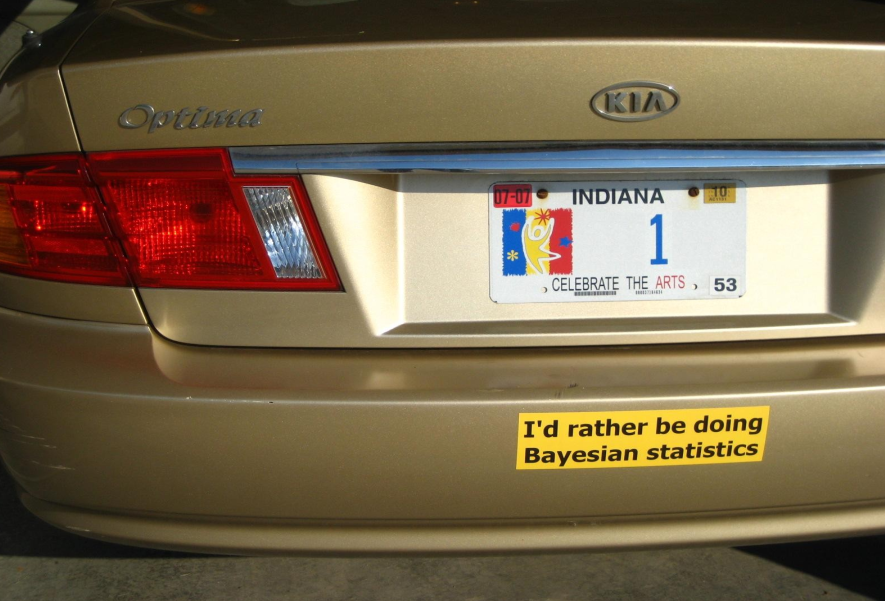
\includegraphics[width=0.6\textwidth]{images/bumper_sticker.png} \\
Credit: John Kruschke
\end{center}

\end{frame}


\begin{frame}
\frametitle{Plan}
\begin{itemize}
\item First we will take a look at an issue involving the use of
probabilities versus probability densities.\pause
\item We will see how to handle multiple data points.\pause
\item Then we will look at {\bf analytic methods}.
\end{itemize}

\end{frame}


\begin{frame}
\frametitle{Computing a Posterior Distribution in R}
Recall the volcano problem, where we had the following assumptions
(prior and sampling distribution respectively) and data,
here written in ``$\sim$'' notation:
\begin{align}
\lambda &\sim \textnormal{Uniform}(0.1, 100) \\
x \given \lambda &\sim \textnormal{Poisson}(\lambda) \\
x &= 20
\end{align}


\end{frame}

\begin{frame}[fragile]
\frametitle{Computing the Posterior Distribution in R}
We represented the uniform prior using the following R vector:
\begin{minted}{r}
lambda = seq(0.1, 100, by=0.1)
prior = rep(1/length(lambda), length(lambda))
\end{minted}
\pause

If we were to make the \mintinline{r}{lambda} grid finer, the probabilities
would get incredibly tiny. It might also be nice to be able to use
\mintinline{r}{dunif()} to make the prior:
\begin{minted}{r}
prior = dunif(lambda, 0.1, 100)
\end{minted}
but this will not sum to 1, because \mintinline{r}{dunif()} returns
probability densities, not probabilities.


\end{frame}


\begin{frame}[fragile]
\frametitle{Probability Densities}
Our new \mintinline{r}{prior} vector created with \mintinline{r}{dunif()}
does not sum to 1, but instead integrates to 1. We can approximate integration
using summation multiplied by the grid spacing to verify this:

\begin{minted}{r}
> lambda = seq(0.1, 100, by=gap)
> prior = dunif(lambda, 0.1, 100)
> sum(gap*prior) # Well, I said it was an approximation!
[1] 1.001001
\end{minted}

We can carry out the entire calculation using densities instead of
probabilities, but every time we do a \mintinline{r}{sum()} we need
to multiply by \mintinline{r}{gap}.

\end{frame}



\begin{frame}[fragile]
\frametitle{Probability Densities}
\begin{minted}{r}
gap = 0.1
lambda = seq(0.1, 100, by=gap)
prior = dunif(lambda, 0.1, 100)
lik = dpois(20, lambda)
h = prior*lik
Z = gap*sum(h)  # Approximately an integral
post = h/Z
plot(lambda, post, type="l")
\end{minted}

\end{frame}


\begin{frame}
\frametitle{Posterior Density}
The values on the $y$-axis are now not tiny, and densities are more appropriately plotted with \mintinline{r}{type="l"}.
\begin{center}
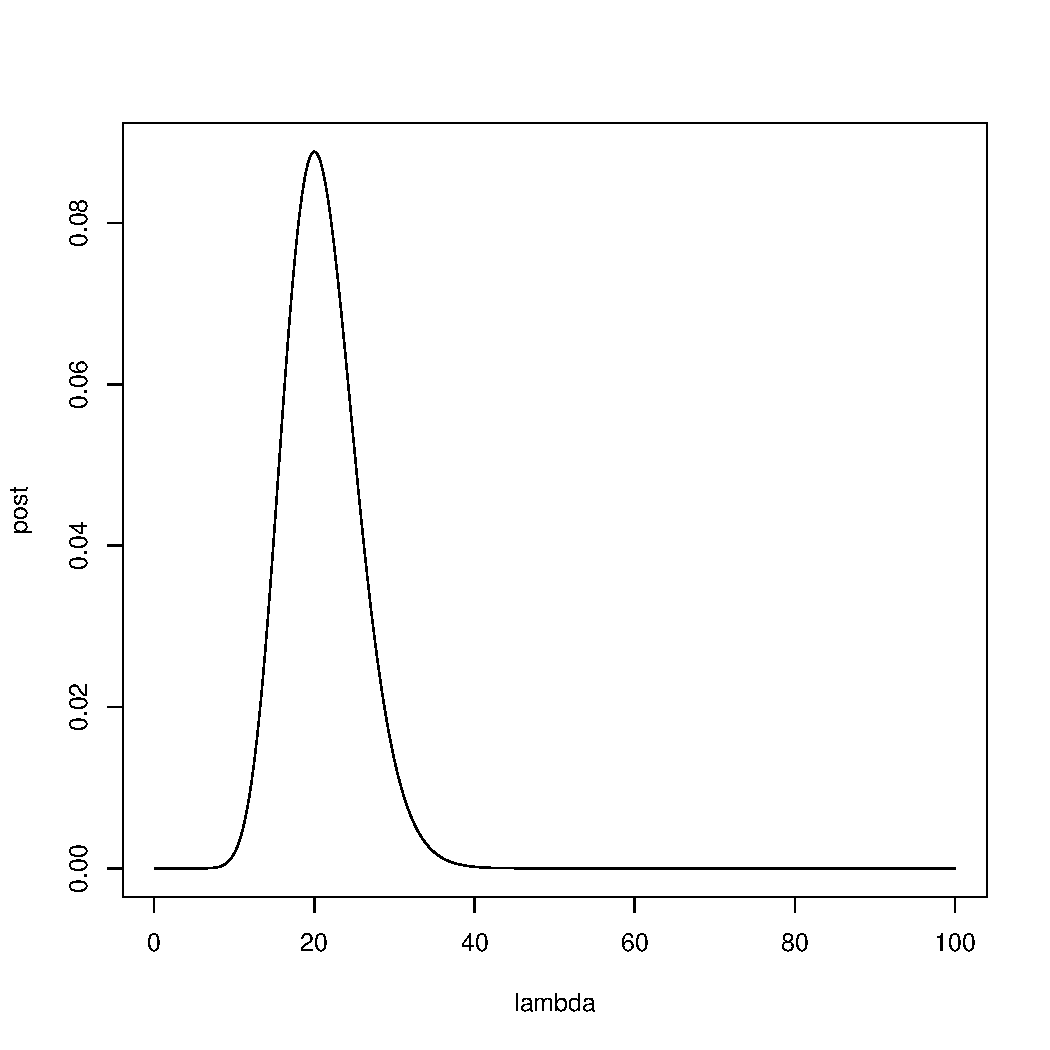
\includegraphics[width=0.35\textwidth]{images/density.pdf}
\end{center}
This method is better if we want to write a prior using
\mintinline{r}{dbeta()} or something (we will see beta distributions soon).

\end{frame}

\begin{frame}
\frametitle{Analytical Methods}

\begin{center}
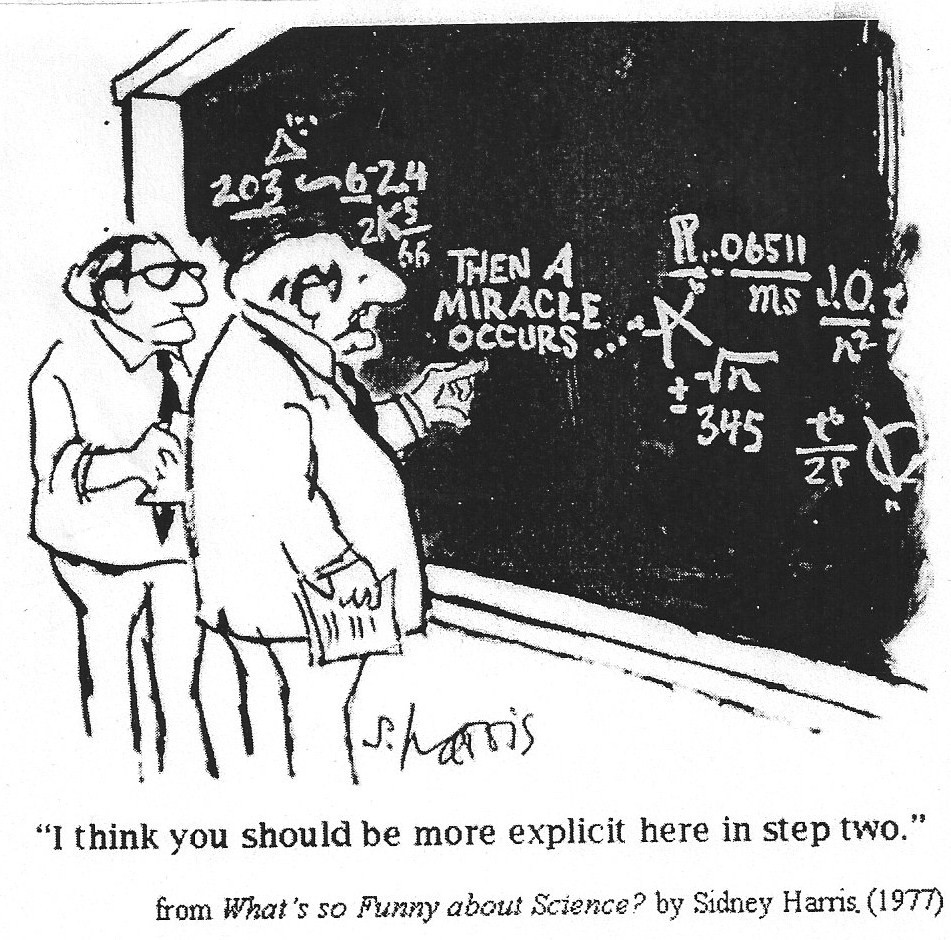
\includegraphics[width=0.6\textwidth]{images/miracle.jpg}
\end{center}

\end{frame}



\end{document}

